\begin{frame}
	\vspace{2cm}
	\begin{center}
		{\Huge\textbf{\textcolor{copenhagenred}{MALA and Barker's Proposal: Gradient-Based MCMC Methods}}}
		\vspace{1cm}

		\rule{4cm}{3pt}
		\vspace{2cm}
	\end{center}
\end{frame}

\begin{frame}{From RWM to more advanced methods}
	\textbf{Random Walk Metropolis (RWM):}
	$$q^* = q + \sigma W, \quad W \sim N(0, I_d)$$

	\textbf{Fundamental Trade-off:}
	\begin{itemize}
		\item Large step-size $\sigma$: Low acceptance
		\item Small $\sigma$: Slow exploration
		\item Optimal: $\sigma = \bigO(d^{-1})$
	\end{itemize}

	\vspace{1em}
	\textbf{Problem:} In high dimensions, RWM becomes inefficient
	\begin{itemize}
		\item Optimal acceptance rate: 0.234
		\item Curse of dimensionality: step size $\propto 1/d$
	\end{itemize}
\end{frame}

\begin{frame}{From Langevin Diffusion to MALA}
	Use gradient to \textbf{move toward modes of $\pi$}

	\textbf{Continuous Langevin Diffusion:}
	$$dX_t = \frac{1}{2}\nabla\log\pi(X_t)dt + dB_t$$

	\begin{itemize}
		\item Has $\pi$ as stationary distribution
		\item Gradient provides moves toward high-probability regions
	\end{itemize}

	\vspace{0.5em}

	\textbf{Euler-Maruyama Discretization (ULA):}
	$$X^{(t)} = X^{(t-1)} + \frac{\epsilon}{2}\nabla\log\pi(X^{(t-1)}) + \sqrt{\epsilon}W$$

	\textbf{Problem} $\pi$ is \textbf{not} the invariant distribution of ULA!

	\textbf{Solution:} Add Metropolis-Hastings correction $\Rightarrow$ MALA
\end{frame}

\begin{frame}{Metropolis-Adjusted Langevin Algorithm \tiny just for reference. do not write down algorithm during exam}
	\begin{algorithm}[H]
		\caption{MALA}
		\begin{algorithmic}
			\STATE \textbf{Input:} Initial $X^{(0)}$
			\FOR{$t = 1, 2, \ldots$}
			\STATE Propose: $X^* = X^{(t-1)} + \frac{\epsilon}{2}\nabla\log\pi(X^{(t-1)}) + \sqrt{\epsilon}W$
			\STATE Compute acceptance ratio:
			$$\alpha = \min\left\{1, \frac{\pi(X^*)q(X^{(t-1)}|X^*)}{\pi(X^{(t-1)})q(X^*|X^{(t-1)})}\right\}$$
			\STATE Accept $X^{(t)} = X^*$ with probability $\alpha$, else $X^{(t)} = X^{(t-1)}$
			\ENDFOR
		\end{algorithmic}
	\end{algorithm}
\end{frame}

\begin{frame}{Optimal Scaling Theory}
	\textbf{Maximizing Expected Squared Jump Distance (ESJD)}
	$\mathbb{E}\left[\|X^{(t+1)} - X^{(t)}\|^2\right]$

	\begin{columns}
		\column{0.40\textwidth}
		\textbf{Dimension Scaling:}
		\begin{itemize}
			\item RWM: $\sigma = \bigO(d^{-1})$
			\item \textcolor{copenhagenred}{MALA: $\sigma = \bigO(d^{-1/3})$}
		\end{itemize}

		\vspace{0.5em}

		\textbf{Optimal Acceptance:}
		\begin{itemize}
			\item RWM: 0.234
			\item \textcolor{copenhagenred}{MALA: 0.574}
		\end{itemize}
		\column{0.5\textwidth}
		\begin{figure}
			\centering
			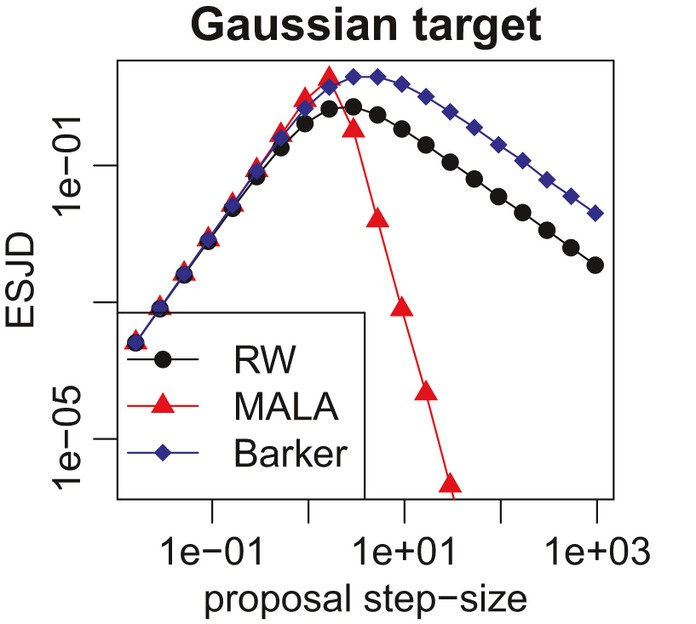
\includegraphics[width=0.6\textwidth]{barker.jpg}
			% \caption{Barker's proposal optimal scaling}
		\end{figure}
	\end{columns}

	\vspace{1em}

	\textbf{Implication:} MALA maintains larger step sizes in high dimensions
	\begin{itemize}
		\item Better exploration efficiency
		\item Faster convergence to target distribution
		\item \textbf{Catch} - requires gradient computation
	\end{itemize}
\end{frame}

% \begin{frame}{From Local-Balanced Proposals to Local-Informed \tiny and back again}
% 	\textbf{General idea:} Start with symmetric proposal $K_\sigma(x,y) =K_\sigma(y,x)$
% 	with step-size $\sigma$ and create informed proposal
% 	$$Q_{\pi}(x,y) \propto \pi(y)K_{\sigma}(x,y)$$
% 	that bias the proposal toward high-probability states. For large $\sigma$ $K_\sigma(x,y) \approx$ Uniform
% 	and when $\sigma$ is tiny, $K_\sigma(x,z) \approx 0$ except when $z$ is near $x$ and in
% 	that case $\pi(x) \approx  \pi(z)$. General form for informed proposals:
% 	$$Q_{g}(x,y) = \frac{g\left( \frac{\pi(y)}{\pi(x)}  \right)K(x,y)}{Z_g(x)}   $$
% 	\textbf{Remarkable result:}, $Q_g$ is \textbf{locally balanced} if $g(t) = tg(1/t)$.
% \end{frame}

\begin{frame}{Building Informed Proposals}
	RWM does not use target information to guide proposals.

	\textbf{Core idea:} Use target density $\pi$ to guide proposals

	\vspace{0.3cm}
	$\textbf{General Framework:} \quad Q_{g}(x,y) = \frac{g\left( \frac{\pi(y)}{\pi(x)}  \right)K(x,y)}{Z_g(x)}$
	
	\vspace{0.3cm}
	where $g$ is a "balancing function".

	\vspace{0.3cm}
	\textbf{Remarkable result:}, $Q_g$ is \textbf{locally balanced} if $g(t) = tg(1/t)$.

	\vspace{0.3cm}
	Two Special Cases:
	\begin{enumerate}
		\item MALA: $g(t) = \sqrt{t}$ 
		\item Barkers Proposal: $g(t) = \frac{t}{1+t}$
	\end{enumerate}
	Both cases satisfy this property. This framework unifies MALA and Barker as different
	choices of the balancing function $g$.
\end{frame}

\begin{frame}{Barker's Proposal}
	Expand $\pi(y)/\pi(x)$ around $x$ with local (first-order) approximation:
	$$e^{\log\pi(y)}  \approx e^{\log\pi(x)+  (\nabla\log\pi(x)^T)(y-x) }$$
	and use $g(t) = t/(1+t)$. This gives $Z_g(x) = 1/2$
	and \textbf{Proposal Density:}
	$$Q_B(x, dy) = \frac{2}{1 + e^{-(\nabla\log\pi(x))^T(y-x)}} K(x, dy)$$
	where $K(x, dy)$ is a base kernel (e.g., Gaussian)

	\textbf{Key Idea:} Use gradient to stochastically bias proposal direction.

	Barker uses gradient to flip coin for direction, MALA uses it as deterministic drift.
	\begin{algorithm}[H]
		\caption{1D case with Gaussian kernel}
		\begin{algorithmic}
			\STATE Sample $Z \sim N(0, \sigma^2)$
			\STATE Calculate $p(x, z) = 1/(1 + \exp(-Z^T\nabla\log\pi(x)))$:
			\STATE Set $b(x,z) = 1$ with probability $p(x,z)$, else $b(x,z) = -1$
			\STATE Propose $Y = x + b(x,z)Z$
		\end{algorithmic}
	\end{algorithm}
\end{frame}

\begin{frame}{Just for my own reference}
	This help to understand why Barker proposal use gradient to
	stochastically bias proposal direction.

	\textbf{Weight of proposal:}
	$$w = \frac{1}{1 + e^{-(\nabla\log\pi(x))^T(y-x)}} = \frac{1}{1 + e^{-g(y-x)}}$$
	where $g = \nabla\log\pi(x)$.

	\textbf{Behavior analysis:} Consider four scenarios based on the signs of $g$ and $(y-x)$:
	\begin{table}[h]
		\centering
		\begin{tabular}{lccccc}
			\toprule
			\textbf{Scenario} & $(y-x)$ & $g(y-x)$ & $e^{-g(y-x)}$ & \textbf{Weight} & \textbf{Meaning} \\
			\midrule
			$g>0$, move right & $>0$    & $>0$     & $\approx 0$   & $\approx 1$     & Favored          \\
			$g>0$, move left  & $<0$    & $<0$     & $\to \infty$  & $\approx 0$     & Penalized        \\
			$g<0$, move left  & $<0$    & $>0$     & $\approx 0$   & $\approx 1$     & Favored          \\
			$g<0$, move right & $>0$    & $<0$     & $\to \infty$  & $\approx 0$     & Penalized        \\
			\bottomrule
		\end{tabular}
		\caption{Barker proposal weight behavior}
		\label{tab:barker}
	\end{table}
\end{frame}

\begin{frame}{MALA vs Barker's Proposal}
	\begin{table}[h]
		\centering
		\begin{tabular}{lll}
			\toprule
			\textbf{Aspect} & \textbf{MALA}                                           & \textbf{Barker}                     \\
			\midrule
			Proposal        & $Y = x + \frac{\sigma^2}{2}\nabla\log\pi(x) + \sigma Z$ & $Y = x \pm Z$ with directional prob \\
			Gradient use    & Drift term (deterministic shift)                        & Direction selection (probabilistic) \\
			% Magnitude & Always adds $\frac{\sigma^2}{2}g$ & Doesn't change $|Z|$ magnitude \\
			Robustness      & Sensitive to step size                                  & More robust to large gradients      \\
			Scaling         & $\bigO(d^{-1/3})$                                       & $\bigO(d^{-1/3})$                   \\
			\bottomrule
		\end{tabular}
	\end{table}
\end{frame}
